\section{Source Code Information}
\figref{code_lines} shows the size of the programs in terms of lines of code. The average number of lines of code for the test suite is @@lines_avg@@, and the median is @@lines_med@@. @@lines_100@@ more than $100$ lines of code, and @@lines_50@@ more than $50$ lines of code.

\begin{figure}[htp]
\centering

\begin{minipage}{.45\textwidth}
    \centering
    \begin{tikzpicture}[scale=0.7]
    
    \selectcolormodel{gray}
    
    \begin{axis}[
        xbar, xmin=0, xmax=250,
        xlabel={Kernel Count},
        symbolic y coords={
            {$> 100$},
            {$81-100$},
            {$61-80$},
            {$41-60$},
            {$21-40$},
            {$<= 20$}
        },
        ytick=data,
        ylabel={Lines of Code},
        nodes near coords,
        nodes near coords align={horizontal},
        height=200pt, width=200pt
    ]
    
    \addplot coordinates {
        (@@lines_100@@,{$> 100$})
        (@@lines_80@@,{$81-100$})
        (@@lines_60@@,{$61-80$})
        (@@lines_40@@,{$41-60$})
        (@@lines_20@@,{$21-40$})
        (@@lines_0@@,{$<= 20$})
    };
    
    \end{axis}
    \end{tikzpicture}
    
    \caption{Lines of Code}
    \label{Fi:code_lines}
\end{minipage}
\hfil
\begin{minipage}{.5\textwidth}
    \centering
    \begin{tikzpicture}[scale=0.7]
    
    \selectcolormodel{gray}
    
    \begin{axis}[
        xbar, xmin=0, xmax=250,
        xlabel={Kernel Count},
        symbolic y coords={
            {$> 400$},
            {$301-400$},
            {$201-300$},
            {$101-200$},
            {$51-100$},
            {$<= 50$}
        },
        ytick=data,
        ylabel={LLVM IR Instructions},
        nodes near coords,
        nodes near coords align={horizontal},
        height=200pt, width=200pt
    ]
    
    \addplot coordinates {
        (@@insts_400@@,{$> 400$})
        (@@insts_300@@,{$301-400$})
        (@@insts_200@@,{$201-300$})
        (@@insts_100@@,{$101-200$})
        (@@insts_50@@,{$51-100$})
        (@@insts_0@@,{$<= 50$})
    };
    
    \end{axis}
    \end{tikzpicture}
    
    \caption{LLVM IR Instructions}
    \label{Fi:llvm_insts}
\end{minipage}

\end{figure}

The instrumentation component of \tool works with LLVM IR and not on the source code. A line of source code could result in zero (e.g., code comments) or more LLVM IR instructions. LLVM IR was generated for @@insts_cnt@@. @@insts_fail@@ did not reach the instrumentation stage of \tool since the compiler could not generate LLVM IR for them. \figref{llvm_insts} shows the size of the programs in terms of LLVM IR instructions. The average number of LLVM IR instructions for the test suite is @@insts_avg@@, and the median is @@inst_med@@.

\begin{figure}[htp]
\centering

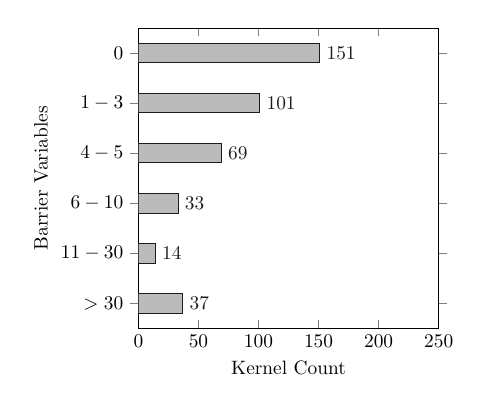
\begin{tikzpicture}[scale=0.7]

\selectcolormodel{gray}

\begin{axis}[
    xbar, xmin=0, xmax=250,
    xlabel={Kernel Count},
    symbolic y coords={
        {$> 30$},
        {$11-30$},
        {$6-10$},
        {$4-5$},
        {$1-3$},
        {$0$}
    },
    ytick=data,
    ylabel={Barrier Variables},
    nodes near coords,
    nodes near coords align={horizontal},
    height=200pt, width=200pt
]

\addplot coordinates {
    (37,{$> 30$})
    (14,{$11-30$})
    (33,{$6-10$})
    (69,{$4-5$})
    (101,{$1-3$})
    (151,{$0$})
};

\end{axis}
\end{tikzpicture}

\caption{Barrier Variables}
\label{Fi:barrier_variables}

\end{figure}


The repair step of \tool depends on the number of barrier variables that have been introduced during instrumentation. \figref{barrier_variables} shows the number of barrier variables introduced in the instrumentation stage of \tool. The average number of barrier variables for the test suite is @@bars_avg@@, and the median is @@bars_med@@.
